% Demo (M2): a Times document (newtx). Left: the figure with Computer Modern outline labels (the default).
% Right: the overlay, whose labels are set by this document in Times.
\documentclass[10pt,twocolumn]{article}
\usepackage[T1]{fontenc}
\usepackage{newtxtext,newtxmath}
\usepackage[textwidth=510pt,columnsep=18pt]{geometry}
\usepackage{graphicx,tikz,contour}
\graphicspath{{../out/}}
\def\cmwdir{../out/}
\begin{document}
\noindent In a Times document the default outline labels are Computer Modern (Fig.~\ref{fig:a}), which a careful reader notices next to Times text: compare the digits $0,1,2$ here. The overlay (Fig.~\ref{fig:b}) sets every label in the document's own font and size, at the cost of one \verb|\input| and the \verb|tikz| and \verb|contour| packages.
\begin{figure}[h]\centering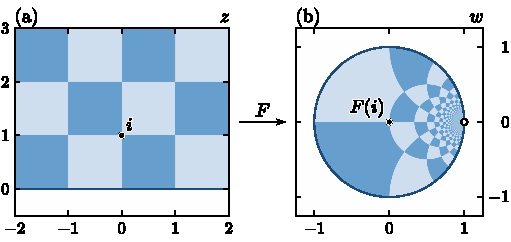
\includegraphics{cayley}\caption{Outline labels (Computer Modern), at natural size in this 246\,pt column.}\label{fig:a}\end{figure}
\begin{figure}[h]\centering% cayley: labels typeset by your document, over cayley-art.pdf. Made for \columnwidth = 246pt.
% Needs \usepackage{tikz,graphicx,amsmath,contour}. If the art lives in a folder, \def\cmwdir{figs/} first.
\providecommand\cmwdir{}
\begin{tikzpicture}[x=1bp,y=1bp,inner sep=0pt,outer sep=0pt]
  \useasboundingbox (0,0) rectangle (245.08,115.95);
  \node[anchor=south west] at (0,0) {\includegraphics{\cmwdir cayley-art.pdf}};
  \node[anchor=north,font=\footnotesize] at (7.00,9.40) {$-2$};
  \node[anchor=north,font=\footnotesize] at (32.71,9.40) {$-1$};
  \node[anchor=north,font=\footnotesize] at (58.43,9.40) {$0$};
  \node[anchor=north,font=\footnotesize] at (84.14,9.40) {$1$};
  \node[anchor=north,font=\footnotesize] at (109.86,9.40) {$2$};
  \node[anchor=east,font=\footnotesize] at (4.50,25.46) {$0$};
  \node[anchor=east,font=\footnotesize] at (4.50,51.17) {$1$};
  \node[anchor=east,font=\footnotesize] at (4.50,76.89) {$2$};
  \node[anchor=east,font=\footnotesize] at (4.50,102.60) {$3$};
  \node[anchor=south west,font=\small] at (60.60,53.35) {\contour{white}{$i$}};
  \node[anchor=north,font=\footnotesize] at (150.86,9.40) {$-1$};
  \node[anchor=north,font=\footnotesize] at (186.86,9.40) {$0$};
  \node[anchor=north,font=\footnotesize] at (222.86,9.40) {$1$};
  \node[anchor=east,font=\footnotesize] at (244.58,21.60) {$-1$};
  \node[anchor=east,font=\footnotesize] at (244.58,57.60) {$0$};
  \node[anchor=east,font=\footnotesize] at (244.58,93.60) {$1$};
  \node[anchor=south east,font=\small] at (184.68,59.78) {\contour{white}{$F(i)$}};
  \node[anchor=base west,font=\small] at (7.00,105.60) {(a)};
  \node[anchor=base east,font=\small] at (109.86,105.60) {$z$};
  \node[anchor=base west,font=\small] at (141.86,105.60) {(b)};
  \node[anchor=base east,font=\small] at (231.86,105.60) {$w$};
  \node[anchor=south,font=\small] at (125.86,60.20) {$F$};
\end{tikzpicture}
\caption{The overlay: labels in newtx Times.}\label{fig:b}\end{figure}
\end{document}
